\documentclass[sigconf,nonacm]{acmart}

\setcopyright{none}
\settopmatter{printacmref=false}
\renewcommand\footnotetextcopyrightpermission[1]{}
\pagestyle{plain}

\usepackage{booktabs}
\usepackage{tabularx}
\usepackage{multirow}
\usepackage{amsmath}
\let\Bbbk\relax
\usepackage{amssymb}
\usepackage{tikz}
\usepackage{pgfplots}
\pgfplotsset{compat=1.18}
\usepackage{url}
\urlstyle{rm}

\usetikzlibrary{arrows.meta,positioning,calc,shapes.geometric,
                decorations.pathreplacing,patterns}

%% ── colour palette ───────────────────────────────────────────────────────────
\definecolor{cblu} {RGB}{ 50,110,190}
\definecolor{cgrn} {RGB}{ 40,150, 70}
\definecolor{cora} {RGB}{210,110, 30}
\definecolor{cred} {RGB}{200, 50, 50}
\definecolor{cyel} {RGB}{190,165,  0}
\definecolor{cpur} {RGB}{130, 50,170}
\definecolor{cgry} {RGB}{100,100,100}

\begin{CCSXML}
<ccs2012>
  <concept>
    <concept_id>10002978.10003006.10003007</concept_id>
    <concept_desc>Security and privacy~Cryptography</concept_desc>
    <concept_significance>500</concept_significance>
  </concept>
  <concept>
    <concept_id>10002978.10003006.10003008</concept_id>
    <concept_desc>Security and privacy~Network security</concept_desc>
    <concept_significance>500</concept_significance>
  </concept>
  <concept>
    <concept_id>10003033.10003106.10003110</concept_id>
    <concept_desc>Networks~Network protocols</concept_desc>
    <concept_significance>300</concept_significance>
  </concept>
</ccs2012>
\end{CCSXML}

\ccsdesc[500]{Security and privacy~Cryptography}
\ccsdesc[500]{Security and privacy~Network security}
\ccsdesc[300]{Networks~Network protocols}

\title{IPsec Security Associations: Architecture, Lifetime Management, and the Security Benefits of Periodic Rekeying}

\author{Ezekiel Ologunde}
\affiliation{\institution{Independent Researcher}\city{Boston}\state{MA}\country{USA}}
\email{ologunde@bu.edu}

\begin{abstract}
IPsec Security Associations (SAs) form the foundational abstraction through which the
IPsec protocol suite delivers confidentiality, integrity, and authentication to IP
traffic. This paper provides a comprehensive treatment of the SA model as specified in
RFC~2401 and RFC~4301, covering the simplex (unidirectional) nature of SAs, the
hierarchical relationship between IKE SAs and child IPsec SAs established by IKEv2
(RFC~7296), and the per-SA keying material that isolates security guarantees across
traffic flows. We analyze SA lifetime management---time-based and volume-based
expiration---and the rekeying process by which implementations replace expiring SAs
without traffic interruption. Through the lens of the CIA triad and forward secrecy,
we demonstrate how periodic rekeying limits cryptanalytic exposure, reinforces
replay protection, and preserves forward secrecy when keying material is refreshed.
We further examine implementation behavior documented in NIST SP~800-77r1, Juniper
Junos, and Fortinet FortiOS, and discuss best practices for SA lifetime configuration,
algorithm agility, and traffic isolation. Our analysis confirms that the simplex,
independent-keying model of IPsec SAs---combined with disciplined rekeying---provides
strong, scalable security for both site-to-site VPN and host-to-host use cases.
\end{abstract}

\keywords{IPsec, Security Association, IKEv2, rekeying, forward secrecy, replay
protection, VPN, cryptographic key management, RFC~7296, NIST SP~800-77}

\begin{document}
\hfuzz=5pt
\maketitle

%%─────────────────────────────────────────────────────────────────────────────
\section{Introduction}
%%─────────────────────────────────────────────────────────────────────────────

Since its standardisation in RFC~2401~\cite{rfc2401} and subsequent revision in
RFC~4301~\cite{rfc4301}, IPsec has become the dominant protocol suite for securing
IP-layer communications. It underpins virtual private networks (VPNs) used by
enterprises, governments, and remote workers worldwide, and provides the foundation
for secure site-to-site interconnection in cloud and hybrid-network architectures.
At the core of every IPsec deployment is the \emph{Security Association} (SA)---a
logical construct that binds a specific set of cryptographic parameters to a
particular traffic flow between two endpoints.

Despite the ubiquity of IPsec, the SA model is frequently misunderstood. Two
misconceptions are especially common. First, practitioners often assume that a single
negotiated SA secures bidirectional traffic; in reality, each SA is strictly
\emph{simplex} (unidirectional), so two SAs are required for full-duplex
communication~\cite{rfc2401}. Second, the relationship between IKE SAs and child
IPsec SAs---and the significance of per-child independent keying material---is often
elided in deployment guides, leading to suboptimal configurations in which all traffic
flows share a single set of session keys.

This paper addresses both misconceptions through a systematic analysis of the SA
architecture, its lifetime semantics, and the security properties conferred by periodic
rekeying. The contributions of this work are as follows:

\begin{itemize}
  \item A formal treatment of the simplex SA model and its implications for
        bidirectional communication, drawing on RFC~2401, RFC~4301, and RFC~7296
  \item An analysis of the IKE SA / child IPsec SA hierarchy and the security
        isolation guarantee that independent keying material provides
  \item A lifecycle model of SA expiration and rekeying, supported by NIST SP~800-77r1
        guidance~\cite{nist80077} and vendor implementation data from Juniper~\cite{juniper}
        and Fortinet~\cite{fortinet}
  \item A security analysis demonstrating how rekeying limits cryptanalytic exposure,
        enforces replay protection, and preserves forward secrecy
  \item Practical configuration guidance for SA lifetime parameters, algorithm agility,
        and traffic isolation across multiple child SAs
\end{itemize}

The remainder of this paper is organised as follows. Section~\ref{sec:background}
reviews the IPsec protocol architecture and the SA database structures.
Section~\ref{sec:sa_model} formalises the simplex SA model.
Section~\ref{sec:hierarchy} examines the IKE SA / child SA hierarchy.
Section~\ref{sec:lifetimes} analyses SA lifetime semantics and the rekeying process.
Section~\ref{sec:security} quantifies the security benefits of periodic rekeying.
Section~\ref{sec:implementation} surveys implementation behaviour across major platforms.
Section~\ref{sec:bestpractices} presents configuration best practices.
Section~\ref{sec:discussion} situates the SA model in broader cryptographic protocol
design. Section~\ref{sec:conclusion} concludes.

%%─────────────────────────────────────────────────────────────────────────────
\section{Background: IPsec Protocol Architecture}
\label{sec:background}
%%─────────────────────────────────────────────────────────────────────────────

\subsection{Protocol Suite Overview}

IPsec is not a single protocol but a suite of components operating at the IP layer.
Figure~\ref{fig:ipsec_arch} illustrates the principal components and their
relationships.

\begin{figure}[h]
\centering
\scalebox{0.84}{
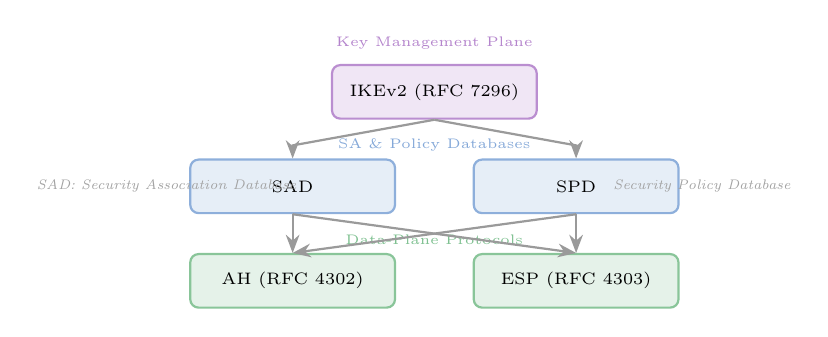
\begin{tikzpicture}[
  font=\fontsize{6.5pt}{8pt}\selectfont,
  >=Stealth,
  box/.style={rectangle, rounded corners=3pt, draw, thick,
              minimum width=2.6cm, minimum height=0.68cm,
              text centered, inner sep=3pt},
  arr/.style={-{Stealth}, thick, cgry!65}
]
  %% Top row: key management
  \node[box, fill=cpur!12, draw=cpur!55] (ike) at (0, 0) {IKEv2 (RFC 7296)};
  \node[font=\fontsize{5.5pt}{7pt}\selectfont, text=cpur!60]
    at (0, 0.62) {Key Management Plane};

  %% Middle row: databases
  \node[box, fill=cblu!12, draw=cblu!55] (sad) at (-1.8,-1.20) {SAD};
  \node[box, fill=cblu!12, draw=cblu!55] (spd) at ( 1.8,-1.20) {SPD};
  \node[font=\fontsize{5.5pt}{7pt}\selectfont, text=cblu!60]
    at (0, -0.68) {SA \& Policy Databases};

  %% Bottom row: data plane protocols
  \node[box, fill=cgrn!12, draw=cgrn!55] (ah)  at (-1.8,-2.40) {AH (RFC 4302)};
  \node[box, fill=cgrn!12, draw=cgrn!55] (esp) at ( 1.8,-2.40) {ESP (RFC 4303)};
  \node[font=\fontsize{5.5pt}{7pt}\selectfont, text=cgrn!60]
    at (0, -1.88) {Data-Plane Protocols};

  \draw[arr] (ike.south) -- (-1.8,-0.68) -- (sad.north);
  \draw[arr] (ike.south) -- ( 1.8,-0.68) -- (spd.north);
  \draw[arr] (sad.south) -- (ah.north);
  \draw[arr] (sad.south) -- (esp.north);
  \draw[arr] (spd.south) -- (ah.north);
  \draw[arr] (spd.south) -- (esp.north);

  %% Labels
  \node[font=\fontsize{5.5pt}{7pt}\selectfont\itshape, text=cgry!60, align=center]
    at (-3.4,-1.20) {SAD: Security Association Database};
  \node[font=\fontsize{5.5pt}{7pt}\selectfont\itshape, text=cgry!60, align=center]
    at ( 3.4,-1.20) {Security Policy Database};
\end{tikzpicture}
}% scalebox
\caption{IPsec protocol architecture. IKEv2 populates the Security Association
  Database (SAD) and Security Policy Database (SPD). AH and ESP consult the SAD
  to apply the cryptographic parameters of the relevant SA to each packet.}
\label{fig:ipsec_arch}
\end{figure}

The two data-plane protocols are:

\textbf{Authentication Header (AH)~\cite{rfc4302}.} AH provides connectionless
integrity and data-origin authentication for IP packets, along with optional replay
protection. It does not provide confidentiality. AH authenticates the IP header in
addition to the payload, which means it is incompatible with Network Address
Translation (NAT).

\textbf{Encapsulating Security Payload (ESP)~\cite{rfc4303}.} ESP provides
confidentiality (encryption), optional integrity, and optional replay protection.
Unlike AH, ESP does not authenticate the outer IP header, making it NAT-traversal
compatible. In practice, ESP is the dominant IPsec data-plane protocol.

\subsection{Security Association Database (SAD)}

The SAD stores the set of active SAs on a node. Each entry in the SAD is keyed by
a triplet $\langle$\textit{SPI}, \textit{Destination IP}, \textit{Protocol}$\rangle$,
where the Security Parameter Index (SPI) is a 32-bit value chosen by the receiving
end and carried in AH or ESP headers to identify the correct SA for inbound packets.
The SAD entry for an SA contains:

\begin{itemize}
  \item Sequence number counter and overflow indicator (replay protection)
  \item Anti-replay window (typically 64 or 1024 packets wide)
  \item AH or ESP algorithm identifiers and associated keys
  \item Lifetime bounds (time and/or byte count)
  \item IPsec protocol mode (Transport or Tunnel)
  \item Path MTU information
\end{itemize}

\subsection{Security Policy Database (SPD)}

The SPD specifies which traffic should be protected by IPsec, bypassed, or discarded.
SPD entries are matched against packet selectors---source/destination IP address
ranges, port ranges, and protocol numbers---to determine the policy action. For outbound
traffic, a policy entry that matches a packet either locates an existing SAD entry
or triggers IKEv2 to negotiate a new SA if none exists.

%%─────────────────────────────────────────────────────────────────────────────
\section{The Simplex Security Association Model}
\label{sec:sa_model}
%%─────────────────────────────────────────────────────────────────────────────

\subsection{Unidirectionality of SAs}

The most fundamental property of an IPsec SA is its unidirectionality. RFC~2401
states explicitly: ``A Security Association (SA) is a \emph{simplex} `connection' that
affords security services to the traffic carried by it''~\cite{rfc2401}. This
architectural choice has important consequences for how bidirectional communication
must be organised.

Figure~\ref{fig:simplex} illustrates the simplex SA pair required for full-duplex
communication between Host~A and Host~B.

\begin{figure*}[t]
\centering
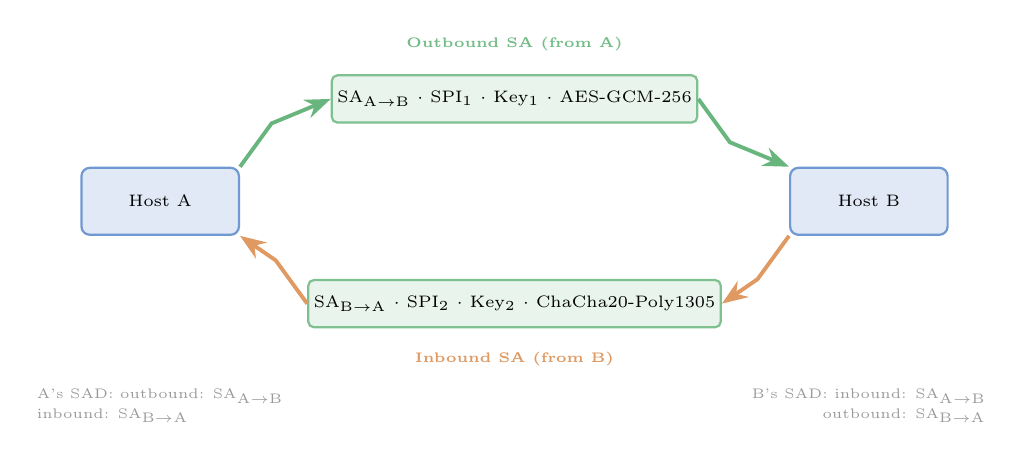
\begin{tikzpicture}[
  font=\fontsize{6.5pt}{8pt}\selectfont,
  >=Stealth,
  host/.style={rectangle, rounded corners=3pt, draw=cblu!70, thick,
               fill=cblu!15, minimum width=2.0cm, minimum height=0.85cm,
               text centered},
  sa/.style={rectangle, rounded corners=2pt, draw=cgrn!60, thick,
             fill=cgrn!10, minimum width=3.5cm, minimum height=0.60cm,
             text centered, font=\fontsize{6pt}{7.5pt}\selectfont, inner sep=2pt},
  arr/.style={-{Stealth}, line width=1.4pt}
]
  \node[host] (A) at (0, 0) {Host A};
  \node[host] (B) at (9, 0) {Host B};

  %% SA-out (A→B): above the midpoint
  \node[sa] (saout) at (4.5, 1.30)
    {SA\textsubscript{A$\to$B} $\cdot$ SPI$_1$ $\cdot$ Key$_1$ $\cdot$ AES-GCM-256};
  \draw[arr, cgrn!70] (A.north east) -- ++(0.4,0.55) -- (saout.west);
  \draw[arr, cgrn!70] (saout.east) -- ++(0.4,-0.55) -- (B.north west);

  %% SA-in (B→A): below the midpoint
  \node[sa] (sain) at (4.5,-1.30)
    {SA\textsubscript{B$\to$A} $\cdot$ SPI$_2$ $\cdot$ Key$_2$ $\cdot$ ChaCha20-Poly1305};
  \draw[arr, cora!70] (B.south west) -- ++(-0.4,-0.55) -- (sain.east);
  \draw[arr, cora!70] (sain.west) -- ++(-0.4,0.55) -- (A.south east);

  %% Labels
  \node[font=\fontsize{5.5pt}{7pt}\selectfont\bfseries, text=cgrn!65]
    at (4.5, 2.00) {Outbound SA (from A)};
  \node[font=\fontsize{5.5pt}{7pt}\selectfont\bfseries, text=cora!70]
    at (4.5,-2.00) {Inbound SA (from B)};

  %% SAD entries
  \node[font=\fontsize{5.5pt}{7pt}\selectfont, text=cgry!65, align=left]
    at (0,-2.60) {A's SAD: outbound: SA\textsubscript{A$\to$B}\\inbound:  SA\textsubscript{B$\to$A}};
  \node[font=\fontsize{5.5pt}{7pt}\selectfont, text=cgry!65, align=right]
    at (9,-2.60) {B's SAD: inbound:  SA\textsubscript{A$\to$B}\\outbound: SA\textsubscript{B$\to$A}};
\end{tikzpicture}
\caption{Simplex SA model for bidirectional IPsec communication. Each SA is strictly
  unidirectional, carrying its own SPI, key material, and algorithm. Full-duplex
  communication between Host~A and Host~B requires two independent SAs with separate
  keys---possibly with different algorithms, as shown here.}
\label{fig:simplex}
\end{figure*}

Each SA owns its own:
\begin{itemize}
  \item \textbf{SPI.} The SPI is chosen independently by each receiving endpoint;
        the SPI in SA\textsubscript{A$\to$B} is chosen by B, and the SPI in
        SA\textsubscript{B$\to$A} is chosen by A.
  \item \textbf{Key material.} Keys are derived independently per SA from the IKEv2
        key derivation function (HKDF-based, defined in RFC~7296), so
        Key$_1 \neq$ Key$_2$ even for the same peer pair.
  \item \textbf{Algorithm suite.} Each SA may independently select its cipher,
        authentication algorithm, and mode, provided both endpoints support the choice.
  \item \textbf{Sequence number counter.} Each SA maintains its own sequence number
        space for replay detection, starting from~1 at SA creation.
  \item \textbf{Lifetime counters.} Time and byte-count lifetimes are tracked
        independently per SA.
\end{itemize}

\subsection{Why Simplex Design?}

The simplex model was a deliberate architectural decision, motivated by the following
considerations.

\textbf{Independent key management.} Inbound and outbound sessions may have different
security requirements in asymmetric deployments (e.g., a client uploading small
requests and downloading large responses). Separate SAs allow independent rekeying
schedules driven by byte-count thresholds.

\textbf{Algorithm negotiation asymmetry.} In early deployments, the two endpoints of a
VPN could be operated by different organisations with different hardware capabilities.
The simplex model allows each direction to be negotiated separately.

\textbf{Replay protection correctness.} Anti-replay windows operate on per-SA sequence
number spaces. A shared bidirectional SA would require a single sequence number space
for packets flowing in both directions, complicating window management for out-of-order
delivery.

\textbf{Failure independence.} If the keying material for one direction is somehow
exposed, the opposing-direction SA is not automatically compromised.

\subsection{Formal SA Identifier}

Formally, an SA is uniquely identified within a node by the 3-tuple:
\[
  \mathrm{SA} \equiv \langle \mathrm{SPI},\ \mathrm{DestinationIP},\ \mathrm{Protocol} \rangle
\]

This means that SPIs from different SAs can coincide provided they differ in
destination address or protocol. Implementations must therefore take care not to
assume global SPI uniqueness when routing inbound packets to their respective SAs.

%%─────────────────────────────────────────────────────────────────────────────
\section{IKE SA and Child SA Hierarchy}
\label{sec:hierarchy}
%%─────────────────────────────────────────────────────────────────────────────

\subsection{IKEv2 Negotiation Phases}

IKEv2 establishes IPsec SAs through a two-phase negotiation process.
Figure~\ref{fig:ike_phases} illustrates the message exchange.

\begin{figure}[h]
\centering
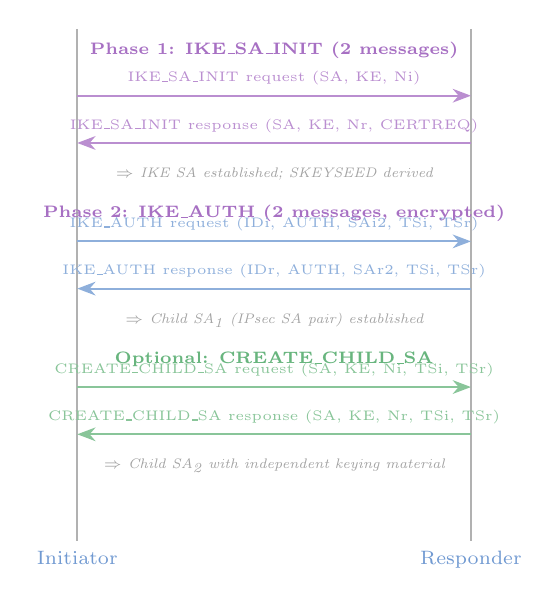
\begin{tikzpicture}[
  font=\fontsize{6.5pt}{8pt}\selectfont,
  >=Stealth,
  msg/.style={-{Stealth}, thick},
  lab/.style={font=\fontsize{5.5pt}{7pt}\selectfont, midway}
]
  %% Vertical lifelines
  \draw[thick, cgry!50] (0, 0) -- (0,-6.5)
    node[below, font=\fontsize{7pt}{9pt}\selectfont, text=cblu!70] {Initiator};
  \draw[thick, cgry!50] (5, 0) -- (5,-6.5)
    node[below, font=\fontsize{7pt}{9pt}\selectfont, text=cblu!70] {Responder};

  %% Phase 1: IKE_SA_INIT
  \node[above, font=\fontsize{6.5pt}{8pt}\selectfont\bfseries, text=cpur!70]
    at (2.5,-0.50) {Phase 1: IKE\_SA\_INIT (2 messages)};
  \draw[msg, cpur!55] (0,-0.85) -- (5,-0.85)
    node[lab, above]{IKE\_SA\_INIT request (SA, KE, Ni)};
  \draw[msg, cpur!55] (5,-1.45) -- (0,-1.45)
    node[lab, above]{IKE\_SA\_INIT response (SA, KE, Nr, CERTREQ)};

  \node[font=\fontsize{5.5pt}{7pt}\selectfont\itshape, text=cgry!60]
    at (2.5,-1.85) {$\Rightarrow$ IKE SA established; SKEYSEED derived};

  %% Phase 2: IKE_AUTH + first child SA
  \node[font=\fontsize{6.5pt}{8pt}\selectfont\bfseries, text=cpur!70]
    at (2.5,-2.35) {Phase 2: IKE\_AUTH (2 messages, encrypted)};
  \draw[msg, cblu!55] (0,-2.70) -- (5,-2.70)
    node[lab, above]{IKE\_AUTH request (IDi, AUTH, SAi2, TSi, TSr)};
  \draw[msg, cblu!55] (5,-3.30) -- (0,-3.30)
    node[lab, above]{IKE\_AUTH response (IDr, AUTH, SAr2, TSi, TSr)};

  \node[font=\fontsize{5.5pt}{7pt}\selectfont\itshape, text=cgry!60]
    at (2.5,-3.70) {$\Rightarrow$ Child SA\textsubscript{1} (IPsec SA pair) established};

  %% Additional child SA
  \node[font=\fontsize{6.5pt}{8pt}\selectfont\bfseries, text=cgrn!70]
    at (2.5,-4.20) {Optional: CREATE\_CHILD\_SA};
  \draw[msg, cgrn!55] (0,-4.55) -- (5,-4.55)
    node[lab, above]{CREATE\_CHILD\_SA request (SA, KE, Ni, TSi, TSr)};
  \draw[msg, cgrn!55] (5,-5.15) -- (0,-5.15)
    node[lab, above]{CREATE\_CHILD\_SA response (SA, KE, Nr, TSi, TSr)};

  \node[font=\fontsize{5.5pt}{7pt}\selectfont\itshape, text=cgry!60]
    at (2.5,-5.55) {$\Rightarrow$ Child SA\textsubscript{2} with independent keying material};
\end{tikzpicture}
\caption{IKEv2 message exchange establishing an IKE SA and two child IPsec SAs.
  Phase~1 (IKE\_SA\_INIT) negotiates Diffie-Hellman parameters. Phase~2 (IKE\_AUTH)
  authenticates peers and creates the first child SA. Additional child SAs can be
  created at any time using CREATE\_CHILD\_SA.}
\label{fig:ike_phases}
\end{figure}

\textbf{Phase 1 --- IKE\_SA\_INIT.} The two IKEv2 messages negotiate the IKE SA
parameters (cryptographic suites), perform a Diffie-Hellman exchange to generate
shared secret material (\texttt{g}\textsuperscript{ir}), and exchange nonces
(\texttt{Ni}, \texttt{Nr}). From these, the IKE master secret \texttt{SKEYSEED} is
derived using the negotiated pseudo-random function (PRF):
\[
  \texttt{SKEYSEED} = \mathrm{PRF}(N_i \mathbin\| N_r,\ g^{ir})
\]
All subsequent IKE messages are encrypted and integrity-protected under keys derived
from \texttt{SKEYSEED}.

\textbf{Phase 2 --- IKE\_AUTH.} The two IKE\_AUTH messages authenticate each peer
(via digital signatures or pre-shared key MACs), exchange traffic selectors
(\texttt{TSi}, \texttt{TSr}), and negotiate the first child SA. The child SA keys
are derived from a separate key stream obtained by expanding \texttt{SKEYSEED} with
additional nonce material, ensuring child keys are cryptographically independent
of the IKE SA's own keys.

\subsection{Multiple Child SAs and Traffic Isolation}

A key architectural feature of IKEv2 is that a single IKE SA can spawn multiple
child SAs, each with its own independent keying material. As documented by the ETH
Zürich IKEv2 analysis: ``it might be beneficial to create additional Child SAs, each
with their own keying material, for instance if the Initiator and Responder want to
communicate with different IP addresses and ports, with a different IPsec protocol,
or if they want to use new improved cryptographic algorithms. Another reason to want
more than one Child SA is to isolate the security guarantees for distinct types of
traffic since IKEv2 ensures that if one of the Child SAs gets compromised, all other
Child SAs are unaffected''~\cite{ethz}.

Table~\ref{tab:child_sa_examples} illustrates practical use cases for multiple child
SAs with traffic isolation.

\begin{table}[h]
\caption{Multiple Child SA Use Cases for Traffic Isolation.}
\label{tab:child_sa_examples}
\small
\begin{tabularx}{\columnwidth}{@{}p{1.7cm}X p{1.5cm}@{}}
\toprule
\textbf{Child SA} & \textbf{Protected Traffic / Purpose} & \textbf{Algorithm} \\
\midrule
SA\textsubscript{1} & Database replication (TCP/5432) & AES-GCM-256 \\
SA\textsubscript{2} & Email transport (TCP/25, 465) & ChaCha20-Poly1305 \\
SA\textsubscript{3} & Management plane (TCP/22) & AES-GCM-128 \\
SA\textsubscript{4} & Bulk data transfer (any/any) & AES-CBC-256+HMAC \\
\bottomrule
\end{tabularx}
\end{table}

If the keying material for SA\textsubscript{2} (email) were ever obtained by an
adversary---through a traffic analysis side-channel, a software vulnerability in
the email processing stack, or a cryptanalytic advance against the negotiated
algorithm---only the email traffic protected by SA\textsubscript{2} would be at risk.
Database replication traffic under SA\textsubscript{1} with its distinct key would
remain protected.

\subsection{Key Derivation Independence}

The independence of child SA keys is enforced by the key derivation structure.
RFC~7296 defines child SA keys as:
\[
  \{K_{\mathrm{enc}}, K_{\mathrm{auth}}, \ldots\} = \mathrm{PRF}^+(\texttt{SK\_d},\ N_i \mathbin\| N_r)
\]
where \texttt{SK\_d} is the child SA key derivation key (itself derived from
\texttt{SKEYSEED} during the IKE SA setup), and $N_i, N_r$ are fresh nonces
contributed by each side during the child SA negotiation~\cite{rfc7296}. Because
each child SA negotiation uses fresh nonces, the derived key material for
SA\textsubscript{1} and SA\textsubscript{2} is statistically independent even if
both are created under the same IKE SA.

%%─────────────────────────────────────────────────────────────────────────────
\section{SA Lifetimes and the Rekeying Process}
\label{sec:lifetimes}
%%─────────────────────────────────────────────────────────────────────────────

\subsection{Lifetime Semantics}

Every IPsec SA is configured with one or both of the following lifetime bounds:

\begin{itemize}
  \item \textbf{Time-based lifetime.} The SA expires after a fixed wall-clock
        duration (e.g., 3600 seconds). This bound prevents long-lived keys from
        accumulating cryptanalytic exposure over time, even on low-traffic links.
  \item \textbf{Volume-based lifetime.} The SA expires after encrypting or
        authenticating a fixed number of bytes (e.g., 4\,GB). This directly limits
        the amount of ciphertext produced under a single key---a central concern
        for cipher modes with restricted nonce spaces.
\end{itemize}

RFC~7296 states: ``IKE, ESP, and AH Security Associations use secret keys that should
be used only for a limited amount of time and to protect a limited amount of data.
This limits the lifetime of the entire Security Association. When the lifetime of a
Security Association expires, the Security Association \textbf{MUST NOT} be used. If
there is demand, new Security Associations MAY be established. Reestablishment of
Security Associations to take the place of ones that expire is referred to as
`rekeying'\,''~\cite{rfc7296}.

Implementations typically define a \emph{soft lifetime} and a \emph{hard lifetime}.
The soft lifetime triggers the rekeying process proactively, before the hard limit
is reached. NIST SP~800-77r1 recommends initiating rekeying when approximately 80\%
of the hard lifetime has elapsed~\cite{nist80077}.

\subsection{The Rekeying Process}

Figure~\ref{fig:rekey} illustrates the SA rekeying process timeline, showing the
old SA (SA\textsubscript{1}), the overlap period, and the new SA (SA\textsubscript{2}).

\begin{figure}[h]
\centering
\resizebox{\columnwidth}{!}{%
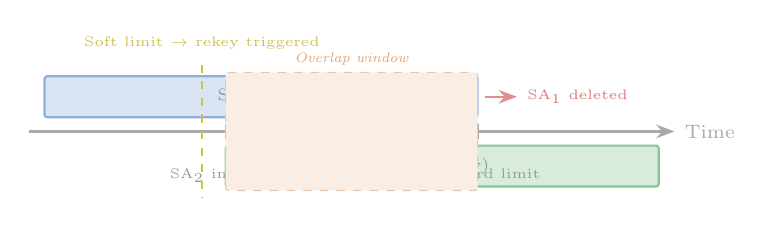
\begin{tikzpicture}[
  font=\fontsize{6.5pt}{8pt}\selectfont,
  >=Stealth
]
  \def\W{7.8}   % total timeline width
  \def\S{0.80}  % soft lifetime x
  \def\H{5.50}  % hard lifetime x

  %% Timeline axis
  \draw[-{Stealth}, thick, cgry!55] (-0.2,0) -- (\W+0.2,0)
    node[right, font=\fontsize{7pt}{9pt}\selectfont] {Time};

  %% SA1 lifespan bar
  \filldraw[fill=cblu!18, draw=cblu!55, thick, rounded corners=1pt]
    (0, 0.18) rectangle (\H, 0.70);
  \node[font=\fontsize{6.5pt}{8pt}\selectfont, text=cblu!70]
    at (\H/2, 0.44) {SA\textsubscript{1} (old)};

  %% SA2 lifespan bar (starts at soft, overlaps until hard)
  \filldraw[fill=cgrn!18, draw=cgrn!55, thick, rounded corners=1pt]
    (\S+1.5, -0.70) rectangle (\W, -0.18);
  \node[font=\fontsize{6.5pt}{8pt}\selectfont, text=cgrn!70]
    at ({(\S+1.5+\W)/2}, -0.44) {SA\textsubscript{2} (new)};

  %% Tick marks
  \draw[thick, cgry!55] (\S+1.5, 0.10) -- (\S+1.5,-0.10);
  \node[below=3pt, font=\fontsize{5.5pt}{7pt}\selectfont, text=cgry!65]
    at (\S+1.5,-0.25) {SA\textsubscript{2} installed};

  \draw[thick, cgry!55] (\H, 0.10) -- (\H,-0.10);
  \node[below=3pt, font=\fontsize{5.5pt}{7pt}\selectfont, text=cgry!65]
    at (\H,-0.25) {SA\textsubscript{1} hard limit};

  %% Soft lifetime marker
  \draw[dashed, cyel!70, thick] (\S+1.2, 0.85) -- (\S+1.2,-0.85);
  \node[above=2pt, font=\fontsize{5.5pt}{7pt}\selectfont, text=cyel!70]
    at (\S+1.2, 0.85) {Soft limit $\to$ rekey triggered};

  %% Overlap shading
  \filldraw[fill=cora!12, draw=cora!40, dashed, rounded corners=1pt]
    (\S+1.5,-0.75) rectangle (\H, 0.75);
  \node[font=\fontsize{5.5pt}{7pt}\selectfont\itshape, text=cora!65]
    at ({(\S+1.5+\H)/2}, 0.92) {Overlap window};

  %% Arrow showing traffic cut-over
  \draw[-{Stealth}, cred!55, thick] (\H+0.1, 0.44) -- (\H+0.5, 0.44)
    node[right, font=\fontsize{5.5pt}{7pt}\selectfont, text=cred!65]
    {SA\textsubscript{1} deleted};
\end{tikzpicture}
}%
\caption{IPsec SA rekeying timeline. When SA\textsubscript{1}'s soft lifetime is
  reached, IKEv2 negotiates SA\textsubscript{2} with fresh keys. Both SAs coexist
  briefly (the overlap window) to prevent traffic disruption. At SA\textsubscript{1}'s
  hard limit, all traffic switches to SA\textsubscript{2} and SA\textsubscript{1} is
  deleted.}
\label{fig:rekey}
\end{figure}

The rekeying process proceeds as follows:

\begin{enumerate}
\sloppy
  \item \textbf{Soft limit reached.} The SA\textsubscript{1} soft lifetime is hit
        (either by time or bytes). The endpoint with the shortest configured lifetime
        (per NIST guidance) initiates a CREATE\_CHILD\_SA exchange over the existing
        IKE SA~\cite{nist80077}.
  \item \textbf{SA\textsubscript{2} negotiated.} A new child SA (SA\textsubscript{2})
        is negotiated with fresh Diffie-Hellman parameters and new nonces. Specifically,
        IKEv2 may include a new KE payload to provide Perfect Forward Secrecy (PFS)
        for the child SA rekey.
  \item \textbf{Overlap window.} SA\textsubscript{2} is installed in both endpoints'
        SADs before SA\textsubscript{1} is torn down. During this window, inbound
        traffic may still arrive on SA\textsubscript{1} (since remote peers may not
        have yet cut over), while outbound traffic can migrate to SA\textsubscript{2}.
  \item \textbf{Hard limit reached / SA\textsubscript{1} deleted.} When
        SA\textsubscript{1}'s hard lifetime is reached, it is removed from the SAD.
        Any inbound packets referencing SA\textsubscript{1}'s SPI are dropped.
  \item \textbf{New SA inherits traffic.} All traffic continues uninterrupted under
        SA\textsubscript{2}'s new keys, new SPI, and fresh sequence number space
        starting from~1.
\end{enumerate}

Fortinet documentation confirms this behavior: ``The purpose of Phase-2 rekeying is to
regenerate the new session keys for Phase-2 SAs; this provides more security to the
associated Child SAs''~\cite{fortinet}.

\subsection{Simultaneous Rekey Race Condition}

RFC~7296 identifies a potential race condition when both peers independently detect
that a child SA requires rekeying at the same moment and each initiates
CREATE\_CHILD\_SA simultaneously. This results in two new SAs being created. The
duplicate detection rule in RFC~7296 specifies that both peers must identify and
delete the SA with the lower \texttt{Nonce} value (where nonces are compared as
unsigned integers), retaining the SA with the higher nonce~\cite{rfc7296}. Correct
implementation of this collision detection logic is essential for avoiding SAD
inconsistency.

%%─────────────────────────────────────────────────────────────────────────────
\section{Security Benefits of Periodic Rekeying}
\label{sec:security}
%%─────────────────────────────────────────────────────────────────────────────

\subsection{Limiting Cryptanalytic Exposure}

The fundamental justification for SA lifetimes is to bound the amount of ciphertext
produced under any single key, thereby limiting the material available to a
cryptanalyst. For a block cipher in CBC mode with a 128-bit block size, the birthday
bound implies that statistical distinguishability becomes feasible after approximately
$2^{64}$ blocks ($\approx$147\,GB) of ciphertext. For AES-GCM, the nonce collision
probability constraint imposes even tighter limits: with a 96-bit random nonce,
nonce collision probability reaches $2^{-32}$ after $2^{32}$ ($\approx$4 billion)
packets under a single key~\cite{rfc4106}.

Volume-based SA lifetimes directly address this by ensuring keys are retired well
below their algorithmic safety limits. Table~\ref{tab:lifetime_guidance} summarises
NIST SP~800-77r1 lifetime recommendations and the cryptographic rationale.

\begin{table}[h]
\caption{Recommended SA Lifetime Parameters (NIST SP 800-77r1).}
\label{tab:lifetime_guidance}
\small
\begin{tabularx}{\columnwidth}{@{}p{1.6cm}X X@{}}
\toprule
\textbf{SA Type} & \textbf{Time Lifetime} & \textbf{Volume Lifetime} \\
\midrule
IKE SA    & 24 hours (max) & N/A (control plane) \\
Child SA  & 1--8 hours (typical) & 100\,MB -- 4\,GB \\
High-security child & $\leq$1 hour & $\leq$100\,MB \\
\bottomrule
\end{tabularx}
\end{table}

\subsection{Forward Secrecy Preservation}

When child SA rekeying incorporates a fresh Diffie-Hellman exchange (i.e., PFS is
enabled), the new session keys are derived from a new ephemeral DH value rather than
from long-lived keying material. This provides \emph{forward secrecy}: an adversary
who later obtains the long-term private key cannot decrypt traffic recorded during
past sessions, because the ephemeral DH values used to protect those sessions are
never stored and therefore irrecoverable.

Without PFS (i.e., when rekeying derives new keys from the existing \texttt{SK\_d}
material via the PRF expansion), forward secrecy is not achieved for child SA
rekeying---compromise of the IKE SA's \texttt{SK\_d} would allow re-derivation of
all child SA keys established under that IKE SA.

\subsection{Replay Attack Mitigation}

Each new SA begins its sequence number counter at~1. The anti-replay window (typically
64 or 1024 packets) tracks the highest received sequence number and maintains a
sliding window bitmask to detect duplicates~\cite{rfc4302}. When SA\textsubscript{1}
is replaced by SA\textsubscript{2}, the sequence number space resets.

This has a direct consequence for replay attacks: any packet captured under
SA\textsubscript{1} carries SA\textsubscript{1}'s SPI. After SA\textsubscript{1} is
deleted from the SAD, the receiving endpoint has no entry for that SPI and will discard
the packet. As Cloudflare's WAN documentation states: ``Replay attacks only work when
attackers use the same encryption keys. After rekeying, the router drops old replayed
packets''~\cite{cloudflare}.

Figure~\ref{fig:replay} illustrates why rekeying eliminates the replay threat window.

\begin{figure}[h]
\centering
\resizebox{\columnwidth}{!}{%
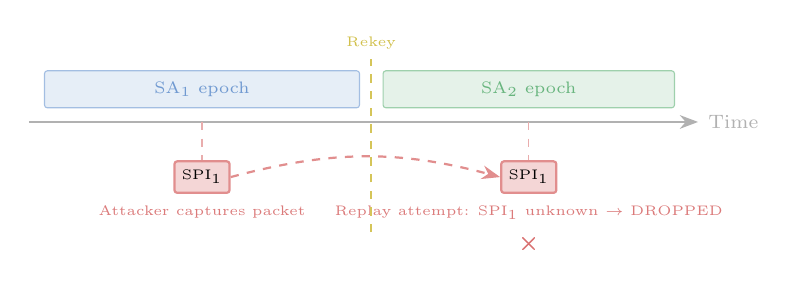
\begin{tikzpicture}[
  font=\fontsize{6.5pt}{8pt}\selectfont,
  >=Stealth,
  pkt/.style={rectangle, rounded corners=1pt, draw, thick,
              minimum width=0.7cm, minimum height=0.40cm,
              text centered, font=\fontsize{5.5pt}{7pt}\selectfont, inner sep=1pt}
]
  %% Timeline
  \draw[-{Stealth}, thick, cgry!50] (0,0) -- (8.5,0)
    node[right, font=\fontsize{7pt}{9pt}\selectfont] {Time};

  %% SA1 epoch
  \filldraw[fill=cblu!12, draw=cblu!45, rounded corners=1pt]
    (0.2,0.18) rectangle (4.2,0.65);
  \node[font=\fontsize{6pt}{7.5pt}\selectfont, text=cblu!70] at (2.2,0.42) {SA\textsubscript{1} epoch};

  %% SA2 epoch
  \filldraw[fill=cgrn!12, draw=cgrn!45, rounded corners=1pt]
    (4.5,0.18) rectangle (8.2,0.65);
  \node[font=\fontsize{6pt}{7.5pt}\selectfont, text=cgrn!70] at (6.35,0.42) {SA\textsubscript{2} epoch};

  %% Captured packet (attacker stores during SA1)
  \node[pkt, fill=cred!20, draw=cred!55] (cap) at (2.2,-0.70) {SPI$_1$};
  \node[font=\fontsize{5.5pt}{7pt}\selectfont, text=cred!65] at (2.2,-1.15)
    {Attacker captures packet};
  \draw[dashed, cred!40] (2.2,0) -- (cap.north);

  %% Replay attempt during SA2
  \node[pkt, fill=cred!20, draw=cred!55] (rep) at (6.35,-0.70) {SPI$_1$};
  \draw[-{Stealth}, cred!55, thick, dashed] (cap.east) to[bend left=15] (rep.west);
  \node[font=\fontsize{5.5pt}{7pt}\selectfont, text=cred!65, align=center]
    at (6.35,-1.15) {Replay attempt: SPI$_1$ unknown $\to$ DROPPED};
  \draw[dashed, cred!40] (6.35,0) -- (rep.north);

  %% Drop marker
  \node[font=\fontsize{8pt}{10pt}\selectfont\bfseries, text=cred!70] at (6.35,-1.55) {\texttimes};

  %% Rekey marker
  \draw[dashed, cyel!65, thick] (4.35,-1.40) -- (4.35,0.80);
  \node[above, font=\fontsize{5.5pt}{7pt}\selectfont, text=cyel!70] at (4.35,0.80)
    {Rekey};
\end{tikzpicture}
}%
\caption{Replay attack prevention through rekeying. A packet captured during
  SA\textsubscript{1}'s epoch carries SPI$_1$. After rekeying, SA\textsubscript{1}
  is deleted and SPI$_1$ is unknown to the receiver, so the replayed packet is
  silently dropped.}
\label{fig:replay}
\end{figure}

\subsection{Key Compromise Isolation}

Even without perfect forward secrecy, the finite SA lifetime limits the damage from a
key compromise. If the session keys for SA\textsubscript{1} are later obtained by an
adversary, only traffic encrypted under SA\textsubscript{1}'s keys---bounded by the
SA's volume and time lifetime---is at risk. Traffic encrypted under the subsequent
SA\textsubscript{2} (with independently derived keys) remains protected.

%%─────────────────────────────────────────────────────────────────────────────
\section{Implementation Behaviour Across Platforms}
\label{sec:implementation}
%%─────────────────────────────────────────────────────────────────────────────

\subsection{NIST SP~800-77r1 Recommendations}

NIST SP~800-77r1~\cite{nist80077} provides comprehensive implementation guidance,
specifying that the gateway with the shortest configured lifetime is responsible for
initiating the rekeying process:

\begin{quote}
\small
``The gateway with the shortest lifetime first determines whether the maximum SA
lifetime is approaching and initiates the rekeying process using the existing IKE
SA. If the IPsec SA is being rekeyed, both ends [install the new SA].''
\end{quote}

NIST further recommends that IKE SA lifetimes should not exceed 24 hours, and that
child SA lifetimes should be significantly shorter to limit exposure on high-throughput
links.

\subsection{Juniper Junos}

Juniper documentation specifies that a Security Association in Junos ``is a simplex
connection that enables two hosts to communicate with each other securely by means of
IPsec. An SA encapsulates the encryption and integrity algorithms, cryptographic keys,
security policy, and the lifetime of the SA. An IKE SA contains attributes for
establishing an IPsec SA whereas an IPsec SA defines the attributes for encrypting the
actual data traffic''~\cite{juniper}. Junos implements the rekeying overlap window by
default, maintaining both the old and new SAs briefly to avoid packet loss during
cutover.

\subsection{Fortinet FortiOS}

Fortinet's IKEv2 implementation provides configurable Phase-2 rekey options. The
default behavior initiates rekeying at 80\% of the hard lifetime threshold.
FortiOS documentation explicitly states: ``The purpose of Phase-2 rekeying is to
regenerate the new session keys for Phase-2 SAs; this provides more security to the
associated Child SAs''~\cite{fortinet}. FortiOS also supports autokey-keep-alive to
maintain SAs in low-traffic scenarios that would otherwise time out prematurely.

\subsection{Open-Source Implementations}

StrongSwan (a widely deployed open-source IKEv2 implementation) and Libreswan both
implement RFC~7296-compliant rekeying. StrongSwan supports marginal time
(\texttt{margintime}) and marginal bytes (\texttt{marginbytes}) parameters that
determine how far in advance of the hard limit rekeying is initiated. Both implementations support PFS for child SA rekeying through configurable DH group selection.

Table~\ref{tab:impl_comparison} compares key SA management features across platforms.

\begin{table}[h]
\caption{SA Lifetime and Rekey Feature Comparison Across Platforms.}
\label{tab:impl_comparison}
\small
\begin{tabularx}{\columnwidth}{@{}p{1.7cm}X X X@{}}
\toprule
\textbf{Feature} & \textbf{FortiOS} & \textbf{Junos} & \textbf{StrongSwan} \\
\midrule
Soft/hard lifetime & \checkmark & \checkmark & \checkmark \\
Volume lifetime    & \checkmark & \checkmark & \checkmark \\
PFS on rekey       & Optional   & Optional   & Optional \\
Rekey overlap      & \checkmark & \checkmark & \checkmark \\
Simultaneous rekey handling & \checkmark & \checkmark & \checkmark \\
Multi-child SA     & \checkmark & \checkmark & \checkmark \\
\bottomrule
\end{tabularx}
\end{table}

%%─────────────────────────────────────────────────────────────────────────────
\section{Best Practices for SA Configuration}
\label{sec:bestpractices}
%%─────────────────────────────────────────────────────────────────────────────

\subsection{Lifetime Parameter Selection}

The selection of SA lifetimes requires balancing several competing concerns:
key exposure (shorter is better), rekeying overhead (shorter increases frequency),
and operational stability (very short lifetimes on high-traffic links can cause
rekeying contention). The following guidelines are based on NIST SP~800-77r1 and
vendor best-practice documentation:

\begin{itemize}
  \item Set IKE SA lifetime between 8--24 hours. Do not allow IKE SAs to persist
        indefinitely, as they protect the re-keying channel itself.
  \item Set child SA time lifetime between 1--8 hours for typical enterprise VPNs.
  \item Set child SA volume lifetime based on link bandwidth. For a 1\,Gbps link,
        a 4\,GB volume limit will be reached in approximately 32 seconds, which is
        far too frequent. NIST recommends volume limits proportional to link capacity
        such that rekeying occurs no more often than every few minutes.
  \item Always enable both time and volume limits. Either limit alone can be
        circumvented: an attacker who can suppress traffic prevents volume limits from
        being reached; an attacker on an idle link benefits from the absence of
        time-based rekeying.
  \item Set the soft limit (rekey initiation) at 80--90\% of the hard limit to ensure
        the overlap window is always available~\cite{nist80077}.
\end{itemize}

\subsection{Algorithm Selection and Agility}

Child SAs should be configured to use AEAD (Authenticated Encryption with Associated
Data) algorithms such as AES-GCM-256 or ChaCha20-Poly1305, which combine
confidentiality and integrity in a single pass and eliminate the CBC+HMAC
combinatorial complexity. NIST SP~800-77r1 deprecates triple-DES and recommends
minimum AES-128-GCM for all new deployments.

The per-SA algorithm negotiation capability should be used to migrate different traffic
streams to stronger algorithms progressively. High-value traffic streams (e.g.,
database replication, management sessions) should be assigned their own child SAs with
the strongest available algorithm suite.

\subsection{Traffic Isolation Strategy}

Deploying multiple child SAs for traffic isolation requires explicit traffic selector
configuration. The traffic selectors (TSi/TSr) in the CREATE\_CHILD\_SA exchange
specify the IP address ranges, port ranges, and protocols that the SA will protect.
Best practices include:

\begin{itemize}
  \item Assign dedicated child SAs to management traffic (SSH, SNMP, RADIUS) with
        stricter lifetime parameters.
  \item Use separate child SAs for traffic from different internal security zones
        (e.g., PCI-DSS cardholder data environment vs.\ general corporate LAN).
  \item Avoid overlapping traffic selectors across child SAs, which can cause
        ambiguous SA selection for outbound packets.
\end{itemize}

\subsection{Perfect Forward Secrecy Considerations}

Enabling PFS for child SA rekeying (by including a KE payload in
CREATE\_CHILD\_SA) is strongly recommended for high-sensitivity deployments. The
additional DH computation cost is modest on modern hardware---a ECDH P-256 operation
requires approximately 0.5\,ms on a contemporary CPU core---and the forward secrecy
guarantee it provides is substantial.

However, PFS must be consistently configured on both peers. Asymmetric PFS
configuration (one end requesting KE, the other not supporting it) can cause rekeying
to fall back to non-PFS mode, silently losing the intended security guarantee. Operators
should verify PFS negotiation success through IKEv2 diagnostic logging.

%%─────────────────────────────────────────────────────────────────────────────
\section{Discussion}
\label{sec:discussion}
%%─────────────────────────────────────────────────────────────────────────────

\subsection{The Simplex Model in Cryptographic Protocol Design}

The simplex SA model represents a deliberate design choice that reflects a broader
principle in cryptographic protocol design: security properties should be established
independently per direction of communication wherever directional parameters can
meaningfully differ. The Transport Layer Security (TLS) protocol applies an analogous
principle through its use of separate write keys for client-to-server and
server-to-client directions. In both cases, the rationale is the same---directional
independence limits the blast radius of a key compromise and simplifies reasoning
about the security properties of each direction.

\subsection{SA Lifetimes and Quantum Threat Posture}

Post-quantum cryptography (PQC) introduces new considerations for SA lifetime
management. Current PQC key encapsulation mechanisms (KEMs) such as CRYSTALS-Kyber
(ML-KEM, FIPS~203) have larger public keys and ciphertexts than classical DH, which
increases the size of IKEv2 key exchange payloads. However, the SA architecture
itself---and the rekeying mechanism---is algorithm-agnostic; replacing the DH
group with a KEM requires only changes to the KE payload handling, not to the SA
lifecycle model.

Internet-Draft draft-ietf-ipsecme-ikev2-ml-kem documents the integration of
CRYSTALS-Kyber into IKEv2. The SA simplex model and rekeying procedures described
in this paper remain fully applicable in post-quantum deployments.

\subsection{Limitations and Open Problems}

\textbf{Rekey contention on high-throughput links.} When volume-based lifetimes are
set too aggressively for high-bandwidth links, the rekeying process can consume
significant control-plane resources, particularly if PFS requires DH computation on
every child SA rekey. Adaptive rekeying mechanisms that monitor link utilisation and
adjust lifetime thresholds dynamically are an open research area.

\textbf{SA proliferation.} Deployments with large numbers of traffic selectors can
result in hundreds of child SAs, each with independent lifetime tracking and rekeying
schedules. Efficient SAD management data structures and rekeying scheduling algorithms
for high-SA-count environments deserve further study.

\textbf{IKE SA compromise.} The current IKEv2 architecture concentrates the key
hierarchy under the IKE SA's \texttt{SKEYSEED}. An adversary who compromises an IKE
SA (not just a child SA) can re-derive all child SA keys established under that IKE SA
(in the absence of PFS). More frequent IKE SA rekeying and mandatory PFS for IKE SA
rekeys mitigate this risk.

%%─────────────────────────────────────────────────────────────────────────────
\section{Conclusion}
\label{sec:conclusion}
%%─────────────────────────────────────────────────────────────────────────────

This paper has provided a comprehensive treatment of the IPsec Security Association
model, from its foundational simplex architecture through the IKEv2-managed child SA
hierarchy to the security benefits of periodic rekeying. The key findings are as
follows.

\textbf{The simplex model is essential, not incidental.} Each IPsec SA is a strictly
unidirectional logical connection. This design choice enables independent key
management, algorithm agility, replay protection correctness, and failure isolation
for each direction of communication. Full-duplex security requires two SAs, each
with its own distinct keying material. This is not a limitation of the protocol but a
deliberate and well-reasoned architectural property.

\textbf{Multiple child SAs provide strong traffic isolation.} A single IKE SA can
spawn multiple child IPsec SAs, each with independently derived keys protecting a
specific traffic class. IKEv2 guarantees that compromise of one child SA does not
affect any other---a guarantee grounded in the cryptographic independence of
per-child key derivation.

\textbf{Rekeying is the primary defence against long-term key exposure.} By retiring
SAs before their algorithmic safety limits are approached, volume-based and time-based
lifetimes bound the ciphertext available for cryptanalysis, reset the anti-replay
sequence number space, and---when PFS is enabled---sever the cryptographic link between
past and future sessions. The rekeying overlap window ensures this lifecycle management
occurs without traffic interruption.

\textbf{Implementation and configuration matter.} The theoretical security properties
of IPsec SAs are fully realised only when operators configure both time and volume
lifetime bounds, enable PFS for child SA rekeying, assign dedicated child SAs to
distinct traffic classes, and verify that soft lifetime thresholds are set sufficiently
far below hard limits to ensure the overlap window is always available.

The IPsec SA model has proven remarkably durable over more than two decades of
deployment, adapting to new algorithms, new threats, and new network architectures
while maintaining the core simplex, finite-lifetime design established in RFC~2401.
Understanding this model in depth is essential for any practitioner responsible for
designing, deploying, or auditing IPsec-based security infrastructure.

\begin{acks}
The author acknowledges the foundational contributions of the IETF IPsec and IKEv2
working groups, whose specifications form the basis of this analysis.
\end{acks}

\sloppy
\bibliographystyle{ACM-Reference-Format}
\begin{thebibliography}{15}

\bibitem{rfc2401}
R.~Kent and R.~Atkinson. 1998. \textit{RFC 2401: Security Architecture for the Internet
Protocol}. Internet Engineering Task Force.

\bibitem{rfc4301}
S.~Kent and K.~Seo. 2005. \textit{RFC 4301: Security Architecture for the Internet
Protocol}. IETF.

\bibitem{rfc7296}
C.~Kaufman, P.~Hoffman, Y.~Nir, P.~Eronen, and T.~Kivinen. 2014.
\textit{RFC 7296: Internet Key Exchange Protocol Version 2 (IKEv2)}. IETF.

\bibitem{rfc4302}
S.~Kent. 2005. \textit{RFC 4302: IP Authentication Header}. IETF.

\bibitem{rfc4303}
S.~Kent. 2005. \textit{RFC 4303: IP Encapsulating Security Payload (ESP)}. IETF.

\bibitem{rfc4106}
J.~Viega and D.~McGrew. 2005. \textit{RFC 4106: The Use of Galois/Counter Mode (GCM)
in IPsec Encapsulating Security Payload (ESP)}. IETF.

\bibitem{nist80077}
K.~Barker, Q.~Dang, S.~Franklin, K.~Scarfone, and P.~Wouters. 2020.
\textit{NIST Special Publication 800-77 Revision 1: Guide to IPsec VPNs}. National
Institute of Standards and Technology.

\bibitem{ethz}
ETH Zürich. 2023. IKEv2 Security Analysis: Child SA Isolation and Rekeying.
Institute of Information Security, ETH Zürich.
\url{https://ethz.ch}

\bibitem{juniper}
Juniper Networks. 2024. Inline IPsec: Security Associations. Junos OS Documentation.
\url{https://www.juniper.net}

\bibitem{fortinet}
Fortinet. 2024. Technical Tip: IPsec Phase-2 Rekey Options and Best Practices.
Fortinet Community Technical Tip.
\url{https://community.fortinet.com}

\bibitem{cloudflare}
Cloudflare. 2024. Anti-Replay Protection. Cloudflare WAN Documentation.
\url{https://developers.cloudflare.com}

\bibitem{rfc6311}
R.~Singh, G.~Kalyani, Y.~Nir, Y.~Sheffer, and D.~Zhang. 2011.
\textit{RFC 6311: Protocol Support for High Availability of IKEv2/IPsec}. IETF.

\bibitem{rfc7427}
T.~Kivinen and J.~Snyder. 2015.
\textit{RFC 7427: Signature Authentication in the Internet Key Exchange Version 2}.
IETF.

\bibitem{nistpqc}
National Institute of Standards and Technology. 2024.
\textit{FIPS 203: Module-Lattice-Based Key-Encapsulation Mechanism Standard (ML-KEM)}.
NIST, Gaithersburg, MD.

\bibitem{rfc9370}
V.~Smyslov. 2023.
\textit{RFC 9370: Multiple Key Exchanges in the Internet Key Exchange Protocol Version 2}.
IETF.

\end{thebibliography}

\end{document}
